\section{Configuring Hardware and Software for the Dot Product Engine}
\label{sec:configDPE}

Advances in computing are often represented by fixed, application specific
hardware. For example, one of the first general purpose computers, The
Electronic Numerical Integrator and Computer (ENIAC), required re-wiring of a
plug board to program it for each application \cite{goldstine1946electronic}.
Likewise, Systolic, Wavefront~\cite{kung1984supercomputing}, and
Dataflow~\cite{iannucci1988toward} architectures each needed to be reconfigured
for a specific computation, such as matrix multiplication or convolution.  Even
Field Programmable Gate Arrays, though reconfigurable, need sophisticated
operating system (OS) support to act as anything more than a fixed system
during operation~\cite{so2006improving}.  Throughout the evolution of these
computing solutions, OS support has been very scarce, relegating these devices
to act as early accelerators and not as general purpose computers.  Even
sophisticated co-processing devices, such as Graphics Processing Units (GPU),
have highly specialized instruction sets that render their use as general
purpose computing resources difficult.

Conversely, OS designers have not easily adapted to the changes in processing
paradigms and increasing importance of power,
largely building systems that rely on a task-based workload model. Although
there have been many notable attempts at building OSes for accelerators, none
of these have been completely successful~\cite{laplante2016rethinking}.

In this study we explore the OS functionality applied to generalizing a
memristor-based accelerator, using a Dot Product Engine (DPE) as an example
that represents an analog form of computer with digital components embedded
into the architecture.  We explore generalizing this accelerator by making it
more reconfigurable and partitionable, as well as more secure.  We also
identify some of the unique characteristics of this kind of system, such as
different precision settings of DPE and trustworthiness of the deployed
configuration into DPE.

\subsection{Background}

\paragraph{Memristor-based Dot Product Engines} Many special-purpose
accelerators have been proposed for neural network
acceleration~\cite{chen2014dadiannao,chi2016prime,shafiee2016isaac}, for which
dot-products are a fundamental operation.  Memristor-based DPEs have been shown
to be particularly promising~\cite{shafiee2016isaac} for computation patterns
(such as inference) where one of the operands is constant and frequently
reused.  The DPE accelerates this operation by programming the constant operand
into a memristor crossbar and performing the computation in-situ with a
streaming input.

\subsection{Dot Product Engine}
\label{sec:DPE}

The Dot Product Engine (DPE)~\cite{hu2016dot} is a hardware accelerator for
matrix-vector multiplication using crossbar arrays to perform highly parallel
multiplications and additions through analog operations.  The concept is not
new~\cite{steinbuch1961lernmatrix,likharev2011crossnets}, with actual
implementations utilizing various technologies such as Flash, phase change
memories (PCM), and oxide-based memristors.  Circuit demonstrations have been
shown in stand alone platforms~\cite{prezioso2015training}, as well as part of
larger programmable analog computing systems~\cite{george2016programmable}.

A full architecture was recently proposed~\cite{shafiee2016isaac} that
integrates analog DPE components in a scalable, pipelined flow with digital
routing, buffers, and other components to flexibly support inference
computations for a broad range of Convolutional Neural Networks (CNN).
Figure~\ref{isaac} shows the basic layout of this architecture, called ISAAC
(In-Situ Analog Arithmetic in Crossbars).  The performance of this architecture
was shown to exceed GPUs and digital ASICs by many orders of magnitude.

At a high level (Figure~\ref{isaac}), an ISAAC chip is composed of a number of
tiles (labeled T), each of which is further composed of eDRAM buffers to store
input values, a number of in-situ multiply-accumulate (IMA) units, and output
registers to aggregate results.  Everything is connected with a shared bus.
Each tile also includes shift-and-add, sigmoid, and max-pool units.  Each IMA
contains several crossbar arrays as well as shared ADCs.

\begin{figure}[t]
\centering
\includegraphics[width=0.9\columnwidth]{ISAAC-CtrlPoints2}
\caption{DPE-based accelerator for convolutional neural
networks~\cite{shafiee2016isaac}.
The DPE can be partitioned by clustering tiles, and control units can be
deployed at different levels.}
\label{isaac}
\end{figure}

Hybrid analog/digital accelerators, such as ISAAC, offer a potential route for
continued growth in focused but important applications while the performance of
general purpose CMOS hardware is flattening.
growth have been proposed, such as quantum, optical, and physical computing.
Using the DPE accelerator as a core example, we highlight some of these
challenges here.

A key performance aspect of the ISAAC architecture is the use of in-memory
processing, whereby memristor arrays not only store neural network weights, but
are also the location for computation. This reduction in data-fetching is a
requirement to realize performance improvements, but it also imposes a strict
data flow that also needs to be pipelined for performance. In ISAAC, a finite
state machine  (expressed as control units in Figure~\ref{isaac}.) is
envisioned to control this data flow needs to be configured by the compiler and
OS. Additionally, portions of the chip can be physically assigned to different
CNNs under computation, possibly at differing priority levels.

In addition to the tile partitioning for a specific task, another
performance-determining parameter is the bit-precision needed in the
matrix-vector multiplication operations. Neural networks are highly tolerant of
low precision~\cite{courbariaux2014low, rastegari2016xnor, zhou2016dorefa}, and
this reduces the burden on the ADCs, which dominate power consumption and
require more time to capture analog signals with higher resolution. Hence, the
precision needed to implement each neural network layer becomes an important
parameter to trade-off performance (high throughput, low power) versus
classification accuracy.  Choosing the optimal operating point requires careful
management.

Mapping neural network layers of various sizes to the appropriate physical
memristor crossbar arrays is another complex management task. As described
above, computations that span multiple physical arrays require additional
peripheral computations to reassemble the aggregate results.  However, simply
placing the neural network layer into the largest possible array can lead to
larger errors (analog signals deteriorate with size and increased non-linear
effects) and slower operating speeds.

The next sections outline how some of the unique trade-offs that are present in
non-traditional, non-digital accelerators and must be managed by OS support
layers.

\subsection{Hardware and Software Autotuning}\label{sec:autotuning}

The configuration of the hardware and software described in this study defines
a large and complex design space and presents an optimization challenge. We
propose to apply autotuning techniques and search heuristics to aid DPE
hardware design and software configuration and optimization.

Changes in hardware and software parameters used to configure the DPE generate
trade-offs and complex parameter relationships. These parameters can be
explored empirically and theoretically.

Table \ref{tab:hard-soft-params} shows hardware and software parameters that
define a design and reconfiguration space for the DPE. The impact of these
parameters on several metrics can be measured using analytical models and
simulations.  Table \ref{tab:metrics-measurements} shows metrics and
measurement strategies that can be optimized for the DPE.

\begin{table}[htpb]
\centering
\begin{tabular}{@{}p{0.46\columnwidth}p{0.46\columnwidth}@{}}
\toprule
\multicolumn{2}{c}{\textit{Tunable Parameters}} \\
\multicolumn{1}{c}{\textit{Hardware}} & \multicolumn{1}{c}{\textit{Software}} \\
Routing tables, eDRAM buffer size; bit size in IMA, layer; bus width; crossbar \& IMA number in tiles & Memristor arrays, layers \& routing tables mapping  \\
\addlinespace
ADC hardware configuration and heterogeneous tile designs & ADC and tile usage \\ \bottomrule
\addlinespace
\end{tabular}
\caption{Tunable software and hardware DPE parameters
}
\label{tab:hard-soft-params}
\end{table}

\begin{table}[htpb]
\centering
\begin{tabular}{@{}p{0.46\columnwidth}p{0.46\columnwidth}@{}}
\toprule
\multicolumn{2}{c}{\textit{Tuning Metrics and Measurements}} \\
\multicolumn{1}{c}{\textit{Metrics}} & \multicolumn{1}{c}{\textit{Measurements}} \\ \midrule
Bandwidth, latency, execution time, router area, throughput & Modelled area and power overhead for components \\
\addlinespace
Computation, power, crossbar efficiency & Cycle accurate simulation for: tile communication; eDRAM access \\
\addlinespace
Usability, flexibility & Empirical, qualitative \\ \bottomrule
\addlinespace
\end{tabular}
\caption{Tuning metrics \& measurement strategies for DPE}
\label{tab:metrics-measurements}
\end{table}

\begin{figure}[htpb]
\centering
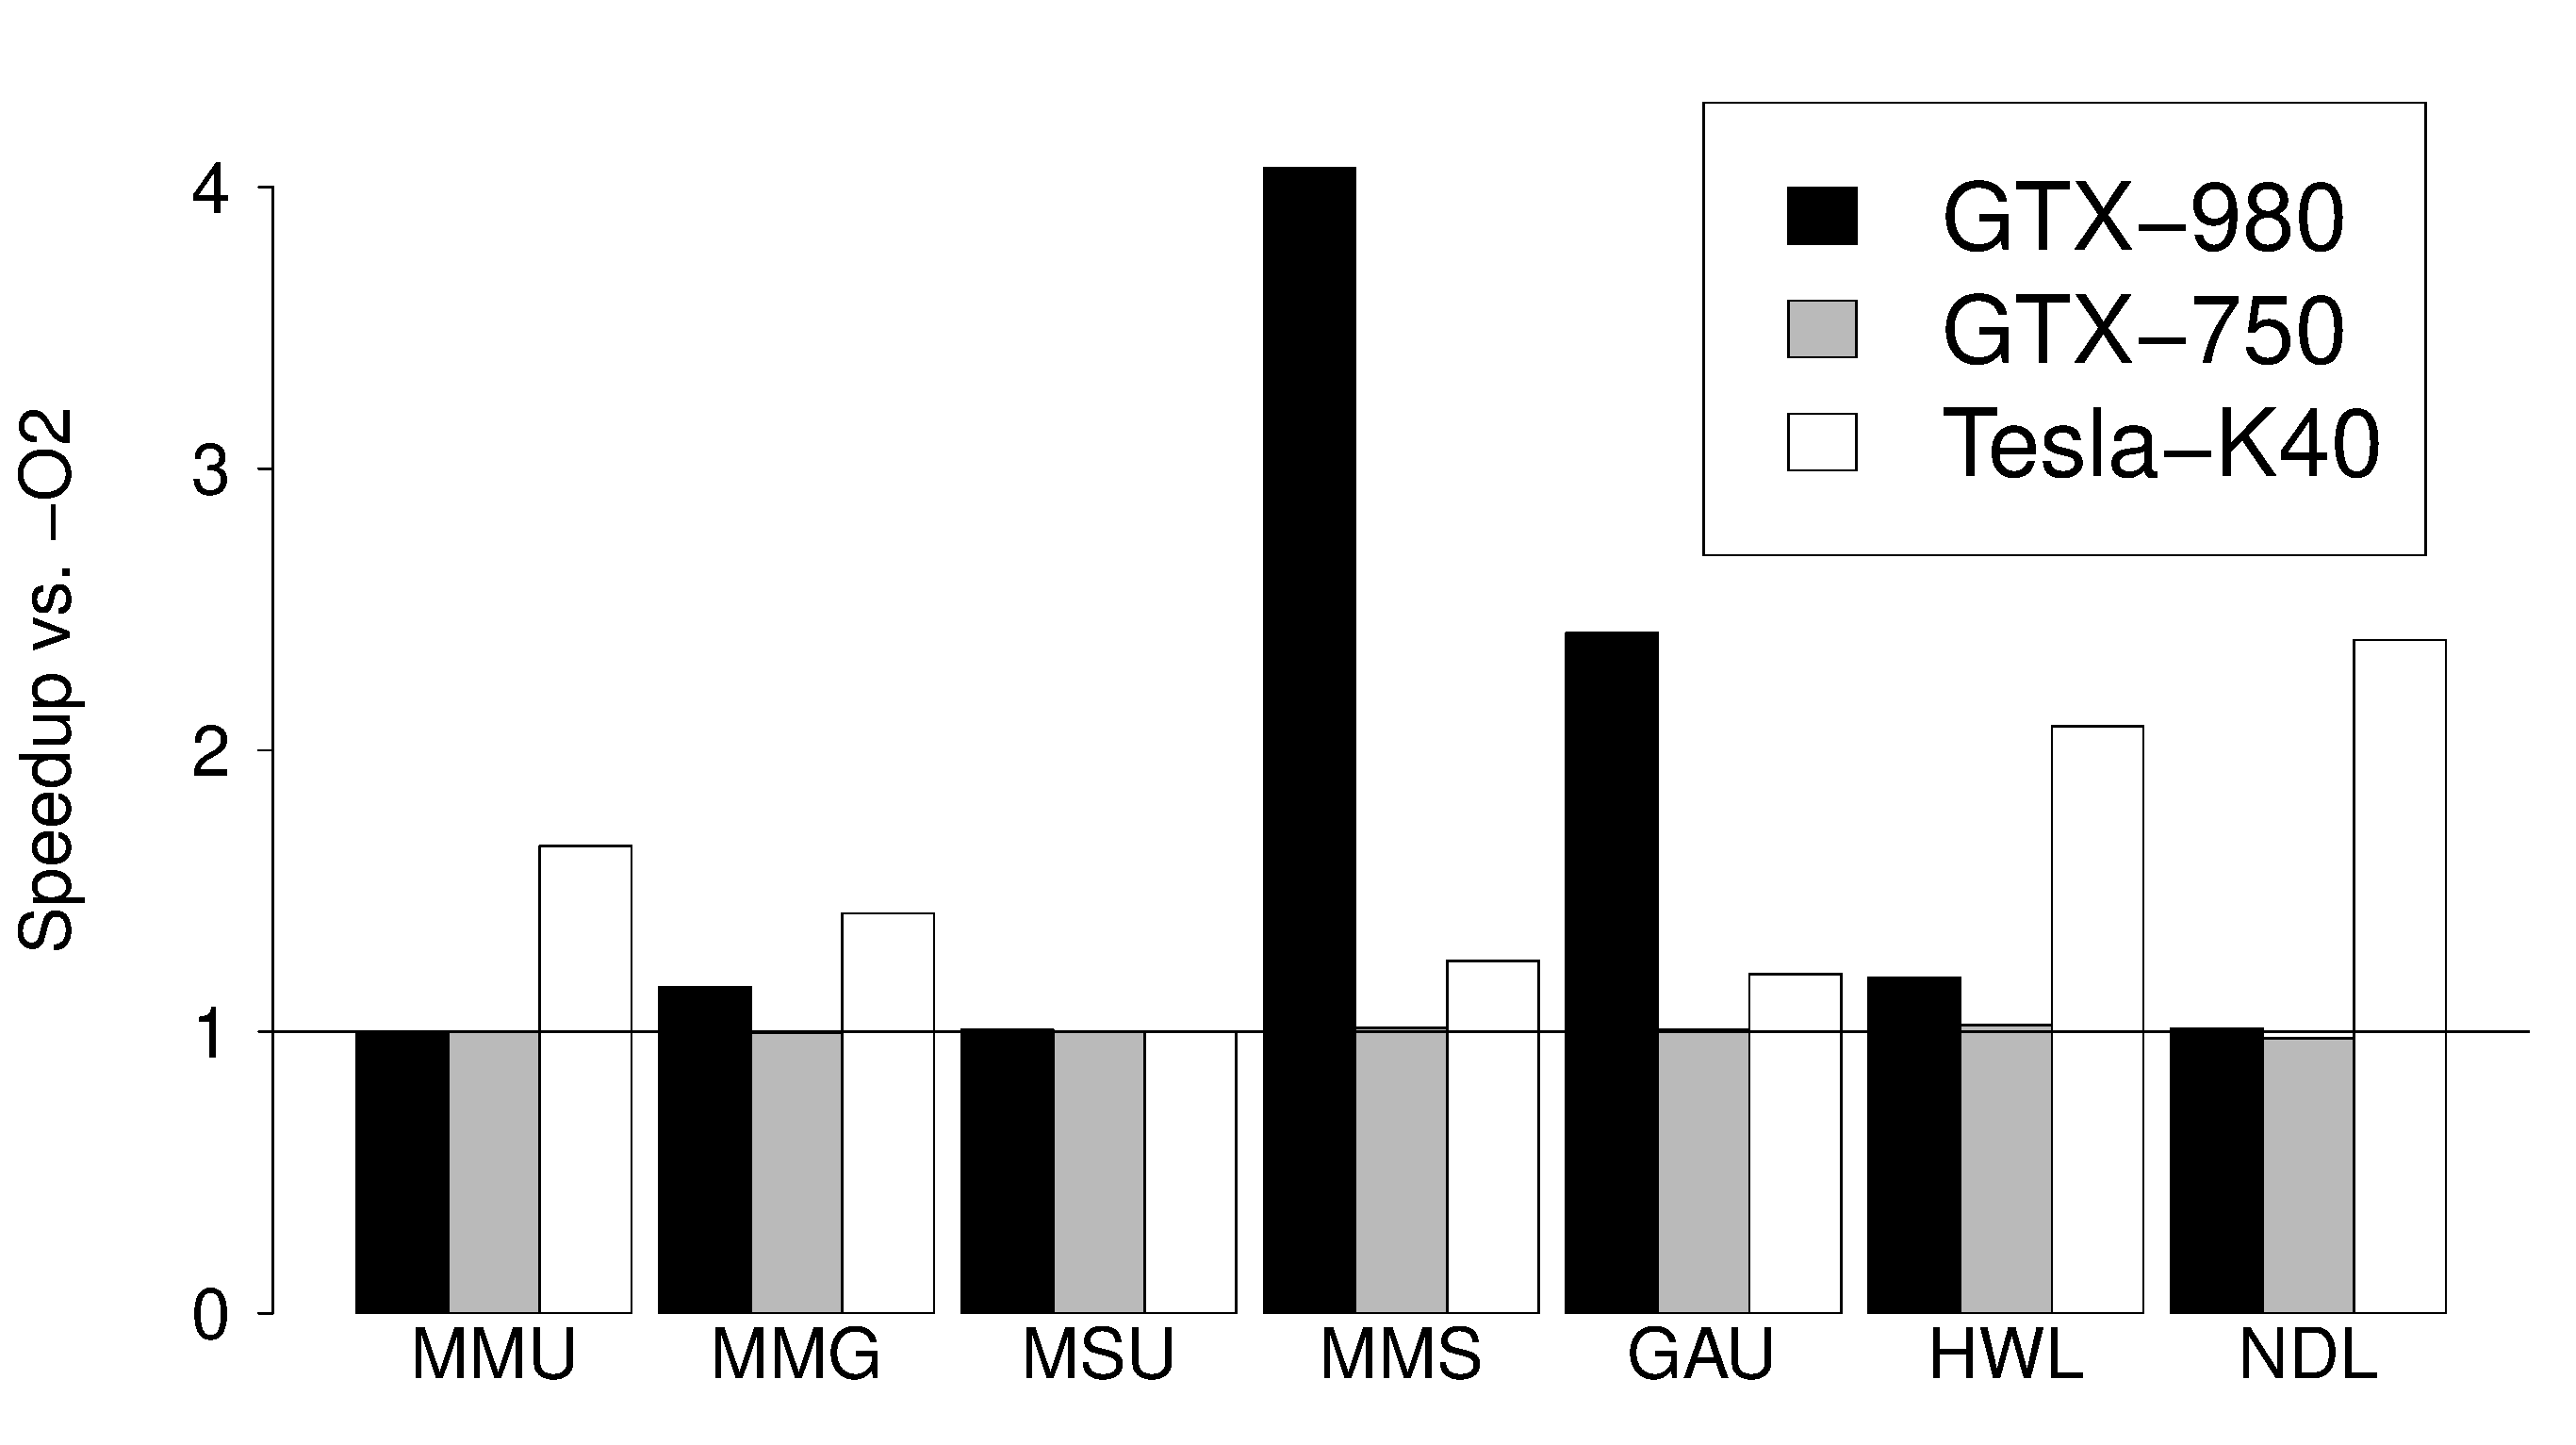
\includegraphics[width=0.9\columnwidth]{GPU-tuning-summary}
\caption{Speedup vs. \texttt{-O2} after autotuning NVCC compiler parameters for heterogeneous
applications~\cite{bruel2017autotuning}}\label{fig:gpu-tuning-summary}.
\end{figure}

\begin{figure}[htpb]
\centering
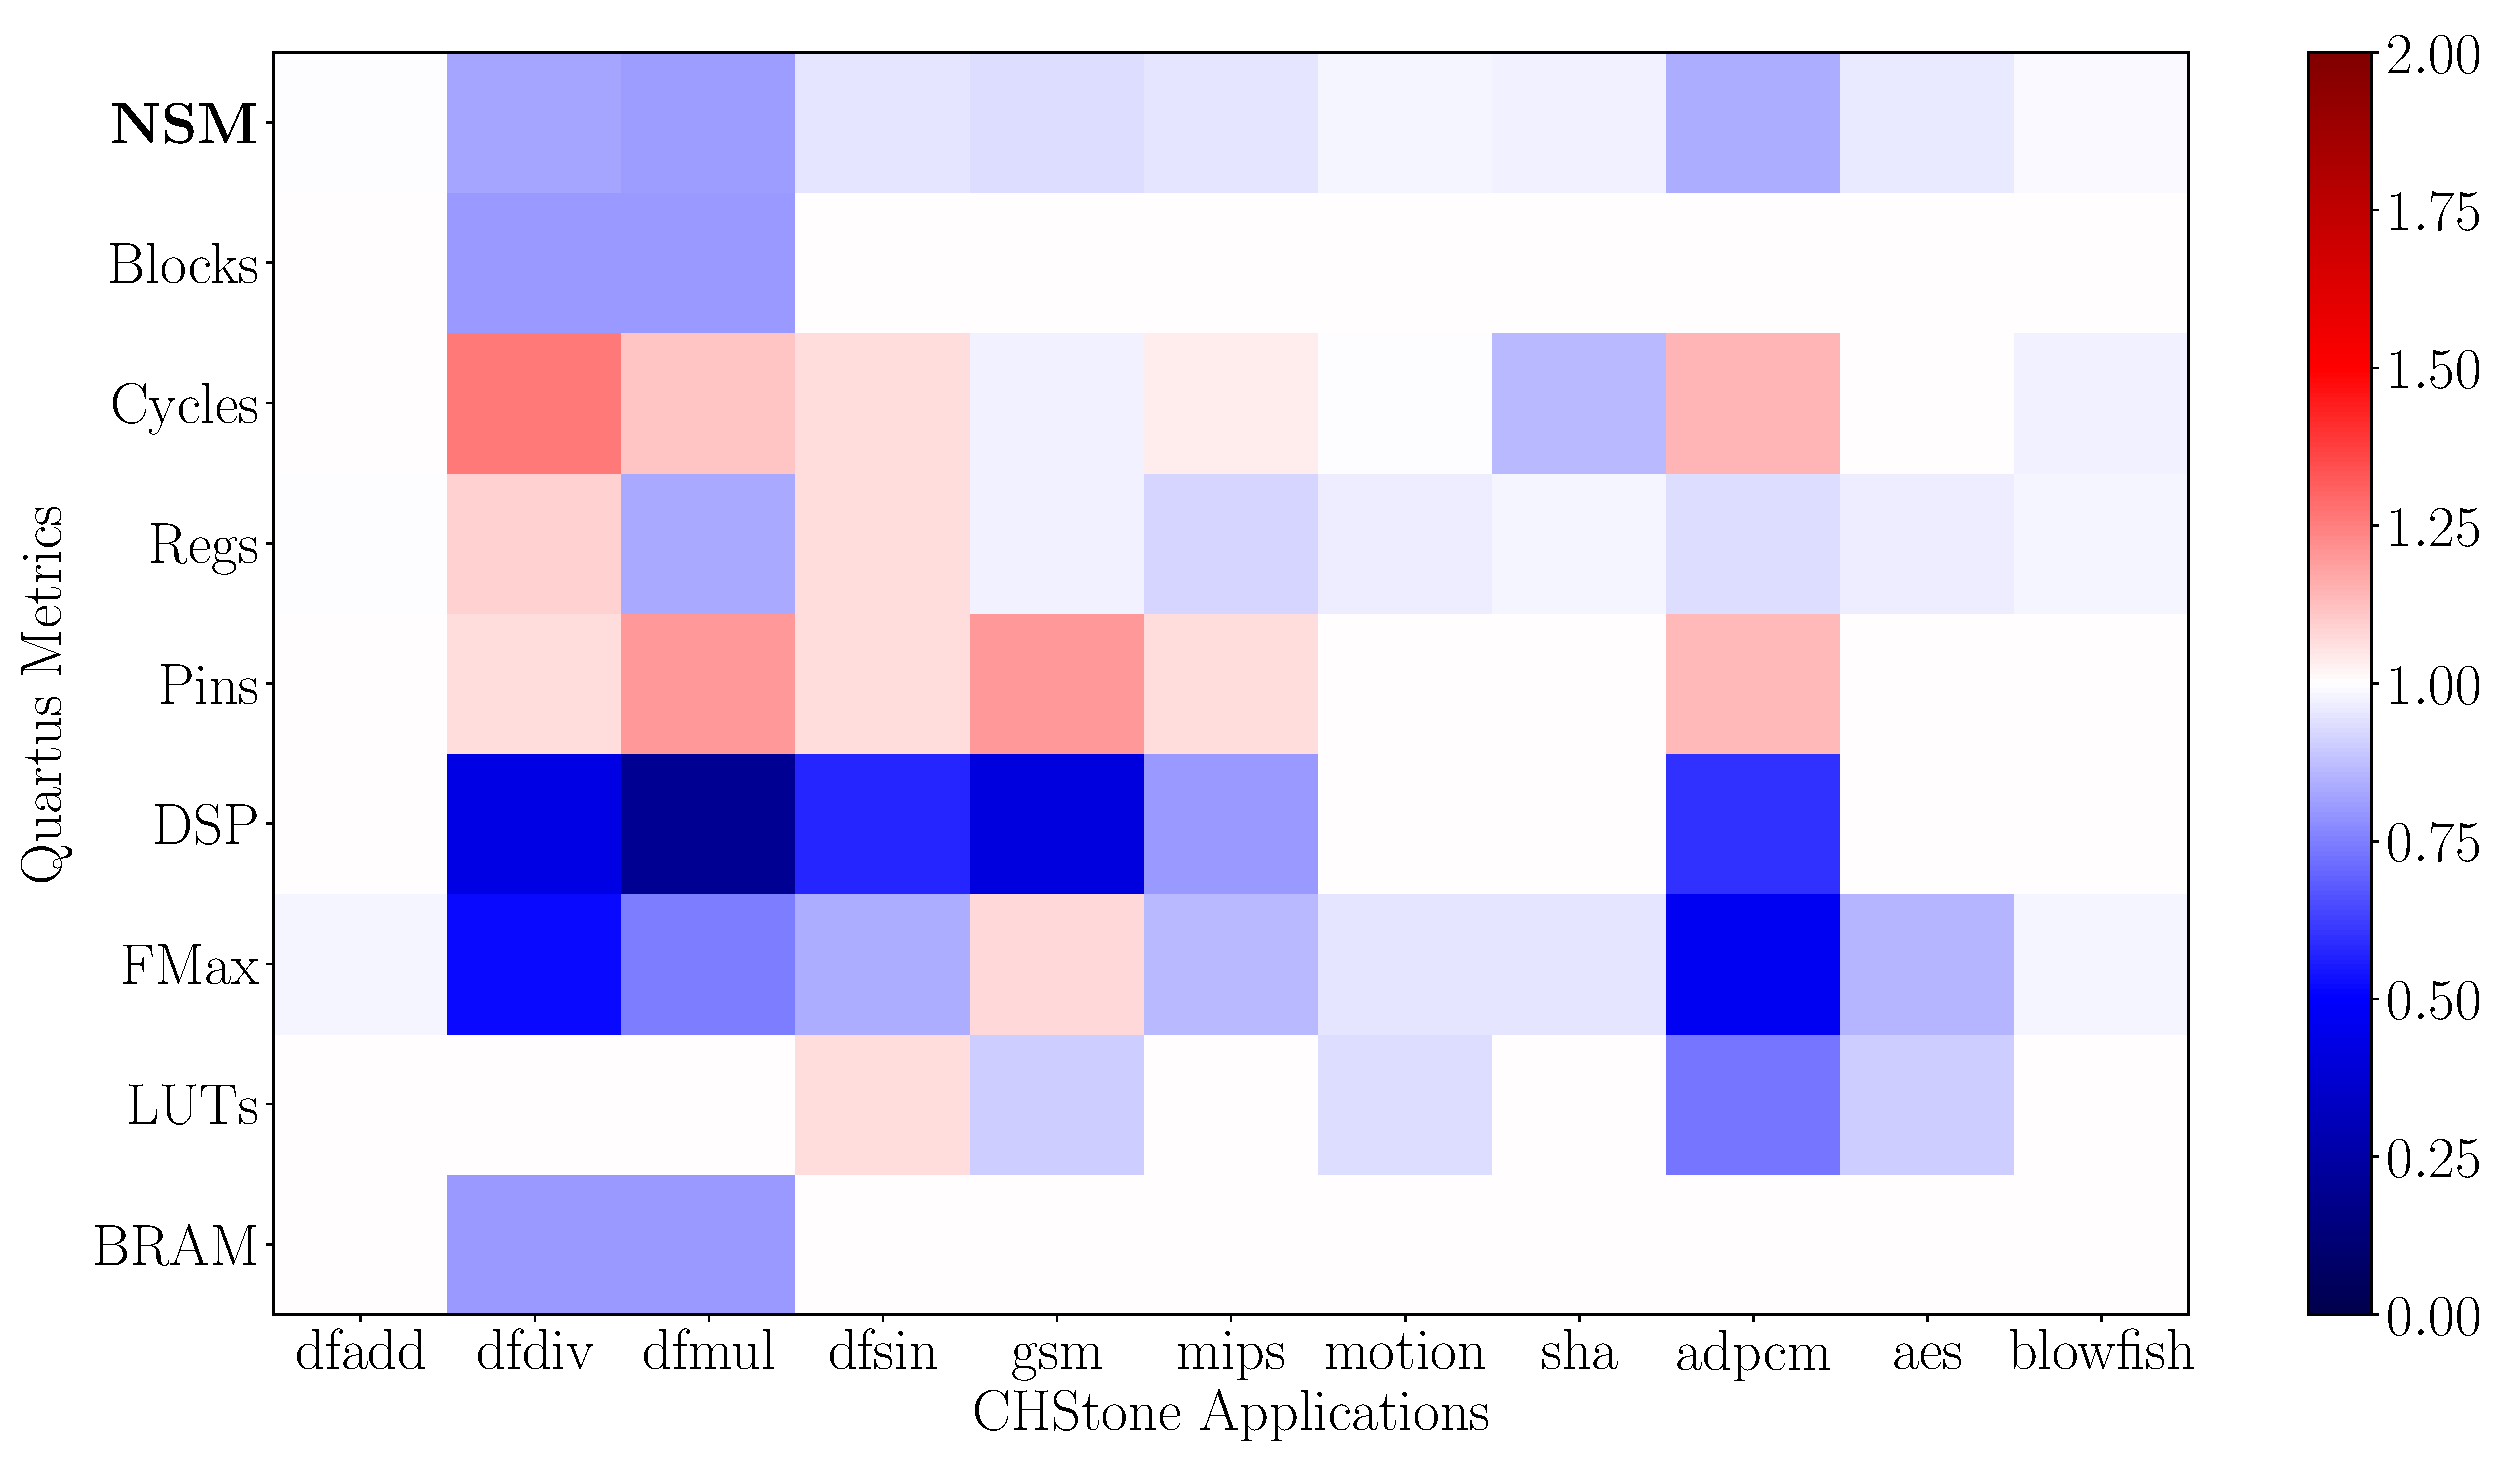
\includegraphics[width=0.9\columnwidth]{FPGA-tuning-summary}
\caption{Relative decrease in Quartus-reported FPGA metrics for CHStone
\cite{hara2008chstone} High-Level Synthesis (HLS)
benchmark.}\label{fig:fpga-tuning-summary}
\end{figure}

For the software configuration, Figure \ref{fig:gpu-tuning-summary} shows the
results \cite{bruel2017autotuning} we obtained using autotuning to optimize the
selection of CUDA compiler flags for Rodinia \cite{che2009rodinia} and matrix
multiplication applications. The applications shown in Figure
\ref{fig:gpu-tuning-summary} are matrix multiplication with uncoalesced access
to global (MMU) and shared memory (MSU), coalesced access to global (MMG) and
shared memory (MMS), gaussian elimination (GAU), heart wall medical imaging
benchmark (HWL) and the Needleman-Wunsh dynamic programming algorithm (NDL).

For the hardware configuration, Figure \ref{fig:fpga-tuning-summary} shows the
results we obtained using autotuning to optimize the configuration of a
High-Level Synthesis (HLS) tool \cite{canis2013legup} subject to a series of
FPGA hardware parameters. The results in Figure \ref{fig:fpga-tuning-summary}
were obtained in the Stratix V DE5-Net FPGA, after tuning HLS parameters. The
intensity of blue squares indicate how much was improved for each metric and
application pair. The autotuning objective was the Normalized Sum of Metrics
(NSM), shown in the first row of the same figure.

Domain-agnostic autotuning frameworks can aid the exploration and optimization
of the DPE hardware and software configurations and design space. We intend to
use this autotuning approach to optimize the DPE parameters listed in Table
\ref{tab:hard-soft-params}, subject to the metrics listed in Table
\ref{tab:metrics-measurements}.

\subsection{Summary and Future Work}
\label{subsec:DPEconcl}
\todo[inline,author=Pedro,color=cyan]{Discuss that the simulator may produce
results very fast. Aayush mentioned that it takes around 2 seconds to simulate
the architecture with pre-generated assembly. It is still unclear for this case.}
